\documentclass{sigchi}

% Use this command to override the default ACM copyright statement
% (e.g. for preprints).  Consult the conference website for the
% camera-ready copyright statement.

%% EXAMPLE BEGIN -- HOW TO OVERRIDE THE DEFAULT COPYRIGHT STRIP -- (July 22, 2013 - Paul Baumann)
 \toappear{Permission to make digital or hard copies of all or part of this work for personal or classroom use is      granted without fee provided that copies are not made or distributed for profit or commercial advantage and that copies bear this notice and the full citation on the first page. Copyrights for components of this work owned by others than ACM must be honored. Abstracting with credit is permitted. To copy otherwise, or republish, to post on servers or to redistribute to lists, requires prior specific permission and/or a fee. Request permissions from permissions@acm.org. \\
{\emph{CHI'14}}, April 26--May 1, 2014, Toronto, Canada. \\
 Copyright \copyright~2014 ACM ISBN/14/04...\$15.00. \\
 DOI string from ACM form confirmation}
%% EXAMPLE END -- HOW TO OVERRIDE THE DEFAULT COPYRIGHT STRIP -- (July 22, 2013 - Paul Baumann)

% Arabic page numbers for submission.  Remove this line to eliminate
% page numbers for the camera ready copy
% \pagenumbering{arabic}

% Load basic packages
\usepackage{balance}  % to better equalize the last page
\usepackage{graphics} % for EPS, load graphicx instead 
\usepackage[T1]{fontenc}
\usepackage{txfonts}
\usepackage{mathptmx}
\usepackage[pdftex]{hyperref}
\usepackage{color}
\usepackage{booktabs}
\usepackage{textcomp}
% Some optional stuff you might like/need.
\usepackage{microtype} % Improved Tracking and Kerning
% \usepackage[all]{hypcap}  % Fixes bug in hyperref caption linking
\usepackage{ccicons}  % Cite your images correctly!
\usepackage[utf8]{inputenc} % for a UTF8 editor only
%\usepackage[utf8]{inputenc}
\usepackage{subfig}

% If you want to use todo notes, marginpars etc. during creation of your draft document, you
% have to enable the "chi_draft" option for the document class. To do this, change the very first
% line to: "\documentclass[chi_draft]{sigchi}". You can then place todo notes by using the "\todo{...}"
% command. Make sure to disable the draft option again before submitting your final document.
\usepackage{todonotes}

% Paper metadata (use plain text, for PDF inclusion and later
% re-using, if desired).  Use \emtpyauthor when submitting for review
% so you remain anonymous.
\def\toolname {Playful Laundry}
\def\plaintitle{\toolname: A Gamified Laundry Booking System}
\def\plainauthor{An Ngoc Lam, An Thien Tran}
\def\emptyauthor{}
\def\plainkeywords{Gamification; Laundry Booking System; Reservation System}
\def\plaingeneralterms{Documentation, Standardization}

% llt: Define a global style for URLs, rather that the default one
\makeatletter
\def\url@leostyle{%
  \@ifundefined{selectfont}{
    \def\UrlFont{\sf}
  }{
    \def\UrlFont{\small\bf\ttfamily}
  }}
\makeatother
\urlstyle{leo}

% To make various LaTeX processors do the right thing with page size.
\def\pprw{8.5in}
\def\pprh{11in}
\special{papersize=\pprw,\pprh}
\setlength{\paperwidth}{\pprw}
\setlength{\paperheight}{\pprh}
\setlength{\pdfpagewidth}{\pprw}
\setlength{\pdfpageheight}{\pprh}

% Make sure hyperref comes last of your loaded packages, to give it a
% fighting chance of not being over-written, since its job is to
% redefine many LaTeX commands.
\definecolor{linkColor}{RGB}{6,125,233}
\hypersetup{%
  pdftitle={\plaintitle},
% Use \plainauthor for final version.
%  pdfauthor={\plainauthor},
  pdfauthor={\emptyauthor},
  pdfkeywords={\plainkeywords},
  bookmarksnumbered,
  pdfstartview={FitH},
  colorlinks,
  citecolor=black,
  filecolor=black,
  linkcolor=black,
  urlcolor=linkColor,
  breaklinks=true,
  hypertexnames=false
}

% create a shortcut to typeset table headings
% \newcommand\tabhead[1]{\small\textbf{#1}}

% End of preamble. Here it comes the document.
\begin{document}

\title{\plaintitle}

\numberofauthors{2}
\author{%
  \alignauthor{An Ngoc Lam\\
    \affaddr{Faculty of Computer Sciences}\\
    \affaddr{Ostfold University College, Norway}\\
    \email{anl@hiof.no}}\\
  \alignauthor{An Thien Tran\\
    \affaddr{Faculty of Computer Sciences}\\
    \affaddr{Ostfold University College, Norway}\\
    \email{antt@hiof.no}}\\
}

\maketitle

\begin{abstract}
This paper describes the approach of gamifying traditional reservation systems for shared facilities in order to improve user experience and usage effectiveness. In particular, we apply the solution to enhance dormitory laundry room usage and present {\toolname} which is a gamified laundry booking system. Similar to any reservation systems,  {\toolname} allows users to reserve washing machines and manage their bookings on mobile phone. Moreover, the system also sends reminders of upcoming booking and finished jobs as well as provides a real time status observation and usage statistics of the machines. Finally, by using game elements: levels, points and leader-board, the systems brings users into playful experiments and changes their behaviors toward efficiently using of the machines. 
\end{abstract}

\category{H.5.2.}{User Interfaces}{Theory and Methods}{}

\keywords{\plainkeywords}

\section{Introduction}

Reservation systems are software systems that store and retrieve information about services or facilities and conduct transactions for booking them. %\cite{wiki:CRS}. 
These systems are most commonly used by airlines or travel agencies to book flight tickets, hotel rooms and lodging facilities. In recent years, there has been a growing trend in sharing ownership of cars, bikes or some other infrequently used assets as a way to avoid paying for such rarely used facilities. In fact, shared-use vehicle systems \cite{barth2002shared, nextbike} have attracted a great deal of interest due to their benefits to the users and environment. Similar to reservation systems, these shared asset management systems not only keep track of resources status and people who are using them but also resolve common problems related to scheduling such as: double or over booking. However, using shared assets involves more than just simply observation and reservation; it is enmeshed in daily activities of users; which constitutes a fluctuation in demand of a particular service or asset. For example, there would be an enormous demand on hotel rooms and airline tickets in holiday seasons; shared vehicles only show their effectiveness before or after working hours. Therefore, the facilities are not used at their highest capacities while the waiting lists are lengthened during peak hours. To keep the number of demands steady, we propose an approach which gamifies traditional reservation systems.

\emph{Gamification}, application of game elements and game principles into non-game contexts to support user engagement \cite{deterding2011game, hamari2014does}, has been applied to improve service use such as increasing social interaction or quality and productivity of the actions \cite{hamari2014does}. In this paper, we aim at understanding how gamification might enhance user experience and change their behaviors in using shared facilities. For evaluation, we present the design and deployment of {\toolname} which is a gamified version of the laundry booking system. Findings from interviewing the students who are currently using a shared laundry room in dormitory offer evidence that our application has attracted much interest of the user and promised to adjust their laundry habits.

\section{Related work}

The idea of a system that affords reservation, observation and notification is not new. It has been widely used in transportation, hotel or even entertainment industries for years. Nowadays, every online reservation systems allows users to reserve services in advance, manage bookings and remind them whenever the time coming. 

There are also some works putting effort on flow optimization such as introducing the concept of ``Reward Pool'' which provides its users with incentives to improve its utilization \cite{winand2006methods}. For example, today most travel reservation systems  award money to the users as an incentive for reserving unpopular time-slots. In \cite{gauld2000solving}, the authors proposed using priority criteria and access threshold in order to remove waiting list of surgical and medical procedures. Edara \emph{et al.} presented Highway Space Inventory Control System which is a booking system for highway trip that determine whether to accept or reject a reservation based on a pre-defined demand in order to optimize the highway allocations for different traffic scenarios \cite{edara2008model}. 

All these solutions are only adaptable for a particular situation and could not be reused at all. In this project, we extend the idea of reservation system toward gamification in order to not only improve user experience but also address the optimization problem.

\section{Gamification and Game Elements}

Gamification has been defined as the use of \emph{game-design elements} for \emph{non-game context} to motivate and improve user activity and retention \cite{deterding2011game, hamari2014does}. Following the success of the location-based services \emph{Foursquare}, the idea of gamification has become a trending topic in interaction design and digital marketing \cite{deterding2011game} in recent years. By using game elements ( points, level and progression, awards, goal/challenge, badges and leader-board, etc. ) as motivational affordances, gamified applications have shown their effectiveness in producing desired \emph{psychological} (e.g., user experience, engagement, fun, etc.) and \emph{behavioral outcomes} (e.g, participation, performance, productivity, etc.) \cite{deterding2011game}. 
%Currently, there is no specified collection of game elements which could be used in gamified systems; it depends on the intentional purpose and the non-game context. Some commonly used elements are: points, level and progression, awards, goal/challenge, badges and leader-board.

There is no doubt that gamification provides effective support for various type of industries. One typical example of gamification  is \emph{Nike+}, a mobile application developed by \emph{Nike}, which successfully motivates people to run. By adding new elements to running, Nike has made running become more fun. With Nike+, users can connect, challenge, cheer and motivate their friends or running buddies around the world. \emph{Xbox Live} is another success example which uses scores, avatars and challenges to involve users into new games. With Xbox Live, \emph{Microsoft} has completely changed console gaming experience for everyone.
 
With the success stories of gamification in motivating users, we hypothesize that this concept is also beneficial to improving the aforementioned situation in current reservation systems.

\section{Laundry Practices}

Laundry practices are not just washing and drying clothes; they are effected by the ordering of
our daily routines \cite{shove2010beyond} and other occasional factors external to laundry itself such as running out of clothes. In order to understand laundry habits and typical use scenarios of shared washing machine, we conducted user surveys and a pilot workshop involving students in the dormitory to collect information about their experiences of using shared laundry room and thinking toward an ideal management system.

It is not very surprising that the students have issues when using the communal laundry room which has a limited number of washing machines. Firstly, to do the laundry, students usually periodically go to the laundry room to check for available machines. During weekend, it could take them hours waiting for their turns. Secondly, the wash times are variable and unpredictable; machines automatically adjust their wash cycle duration according to factors such as: clothes weight, water temperature or pressure, etc. Therefore, students also have to check for the finished jobs. Sometimes, forgetting to pick up the clothes could get them left out by other student. However, these situations only happen commonly during peak hours when the vast majority of students come and do their laundry at the same time whereas the washing machines are being left unused at other times; resulting in an inefficient usage of the machines.

With those aforementioned issues of an example of ``the tragedy of the commons'' at the dormitory, the participants in the workshop also come up with some requirements for a management system. Particularly, they are looking forward to a system that allows them to reserve laundry time-slot in advance and remind them for upcoming booking or finished job. Some students do not always remember to book a time-slot, they want the system to allow them to reserve the machine at the laundry room or provide information about available machine right away without having to go to the laundry room.

Based on the collected information and envisioning, we design and prototype {\toolname}, a laundry booking system which affords:
\begin{itemize}
\item Reserving and managing time-slot on mobile phone or at the laundry room.
\item Notifying the users for upcoming bookings, finished jobs.
\item Real-time status observation of the machines.
\item Display of statistics about usage history of the machines.
\end{itemize}

\section{Our Approach}

\subsection{The Game Rules}

Based on the information collected from users and \emph{envisioning}, we have designed and prototyped {\toolname}, a laundry booking system which affords:
\begin{itemize}
\item Reserving and managing time-slot on mobile phone or at the laundry room.
\item Notifying the users of upcoming bookings, finished jobs.
\item Real-time status observation of the machines.
\item Display of statistics about usage history of the machines.
\end{itemize}
Additionally, \emph{avatars}, \emph{points}, \emph{level/progress} and \emph{leader board} are added in order to make doing laundry more dramatic.

\emph{Avatar} is a graphical representation of a user. Users are not required to add an avatar image. If they do, their avatars could appear along with their rankings on the leader board. 

\emph{Leader board} shows user names, avatar, levels and their ranks among other users. Leader board ranks users based on their current levels and progressions. By default, the system shows only top twenty users on the leader board.

\emph{Level} is used for ranking users. The users need to earn some points in order to get to the next level. They are also awarded points for leveling up. The amount of required points keeps increasing with the level number. In exchange for that, they also get bigger awards. In addition, there is also limitation on the number of reservations (per week) that users allows to make. This number would increase when the users get to higher levels. Progression signifies the percentage of points users already get over the required points they need for getting to the next level. Whenever some users are at the same level, progressions are used to determine their ranks on the leader board.
 
Typically, a laundry booking system allows users to reserve a washing machine for a period of time. They also have to pay for that reservation by cash. With {\toolname}, users can also make reservations with their points. However, earning some points is not easy whereas it costs much more points, compared with a smaller amount of money, to book a machine. The users can earn points by:
\begin{itemize}
\item Making reservations. The users earn some points for each time they book a machine. However, the amounts of awarded points are not the same for every time-slot. Booking in unpopular time-slots would get them more points. Every week, the system calculates statistics about the bookings made in that weeks by hours and days; based on these numbers, it would determine and assign points to each time-slot on the principle of balancing the amounts of bookings in each time-slot.
\item Leveling up. The users would get some points when getting to a new level. The higher level, the more awarded points.
\item Being in top twenty of the leader board. Every week, the system would award some points to users whose names are shown on the leader board. The higher rank, the bigger award.
\item Reporting. By reserving a machine, the users are responsible for finishing their job within a period of time. However, if they forget to pick up their clothes, other users could report them as being late. They would lose some points for the person who has reported them.
\end{itemize}

\subsection{Prototype}

Based on the presented idea, we design and present the prototype which consists of three components (see Figure \ref{fig:figure1}):
\begin{itemize}
\item The server centrally manages all users information, bookings and machines status.
\item Each washing machine has a monitoring device which displays current states of the machine and communicate with server.
\item {\toolname} is the laundry booking application on mobile phone.
\end{itemize}
\begin{figure}[h]
\centering
  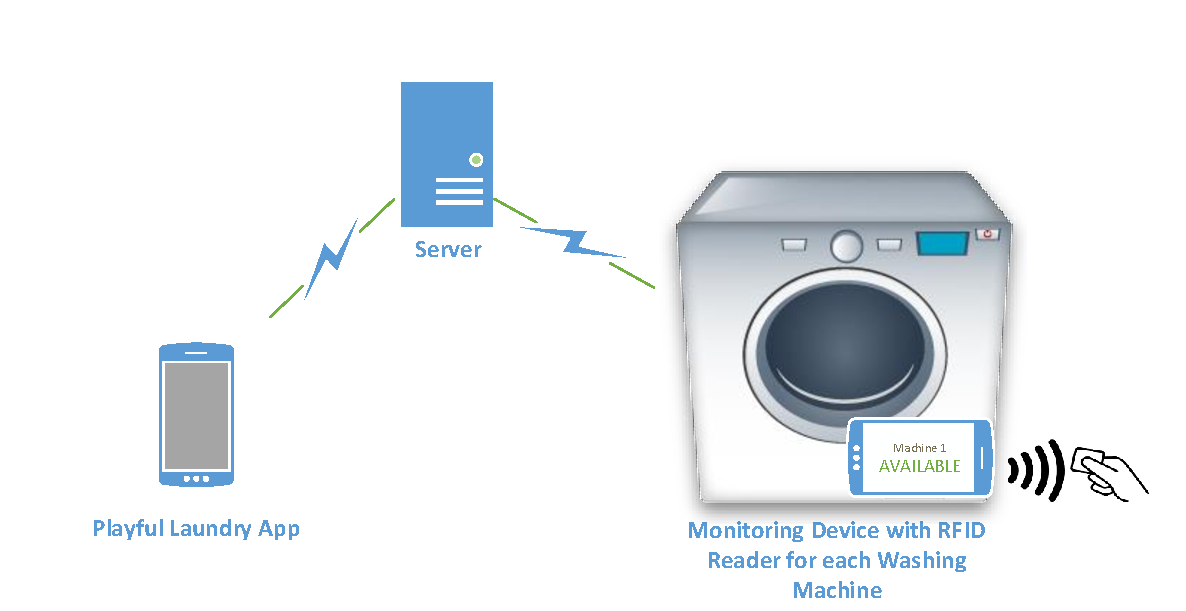
\includegraphics[width=\columnwidth]{figures/overview}
  \caption{Three components of the booking system.}~\label{fig:figure1}
\end{figure}
\subsubsection{Monitoring Device}
Each monitoring device has a RFID reader and a screen which displays interactive instructions and information of the machine such as: machine id, remaining time of current job, current state of washing machine (\emph{AVAILABE} - there is still enough time before the next reservation begins, \emph{USED IN A MOMENT} - next reservation will begin shortly, \emph{RESERVED} - the machine was already booked at that moment, \emph{IN USE} - machine is running, \emph{FINISHED} - washing has just finished), etc.
 For prototyping monitoring device, we use an android phone as a display and an arduino uno board with RFID shield (see Figure \ref{fig:figure2}).
\begin{figure}[h]
\centering
  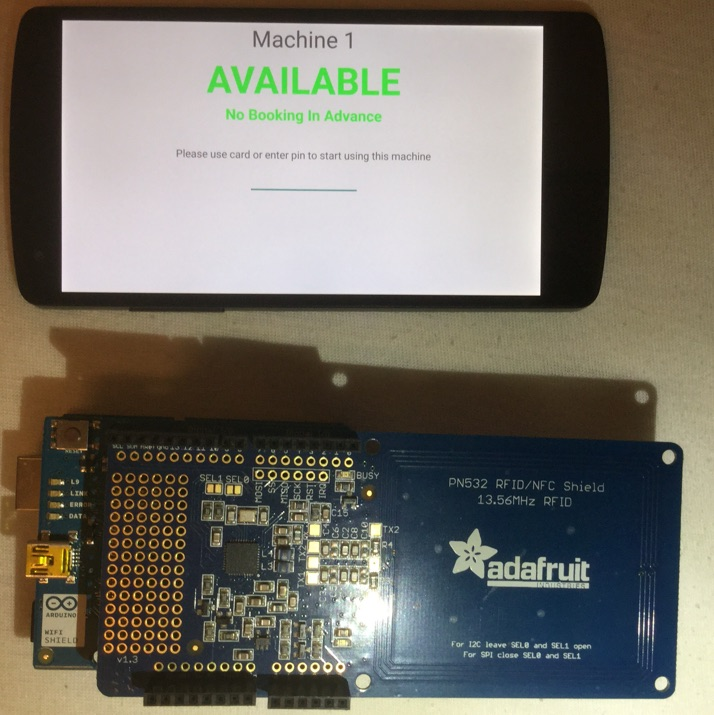
\includegraphics[width=0.7\columnwidth]{figures/Monitoring}
  \caption{The prototype of monitoring device.}~\label{fig:figure2}
\end{figure}
To activate a machine, users could either scan their RFID cards or enter PIN number. If the users already reserved the current time-slot, monitoring device would instruct them to start the machine; otherwise they have to go through booking process right on the monitoring device before using the machine.

When the machine is \emph{IN USE} or \emph{FINISHED} state, the \emph{booking id} of current session would be shown on the screen. Figure \ref{fig:figure3} shows the screenshot of the display when the machine is \emph{IN USE}. This id disappears once the users take their clothes out of the machine. Therefore, if the users are being late, other users could use this \emph{booking id} and the \emph{machine id} for reporting.
\begin{figure}[h]
\centering
  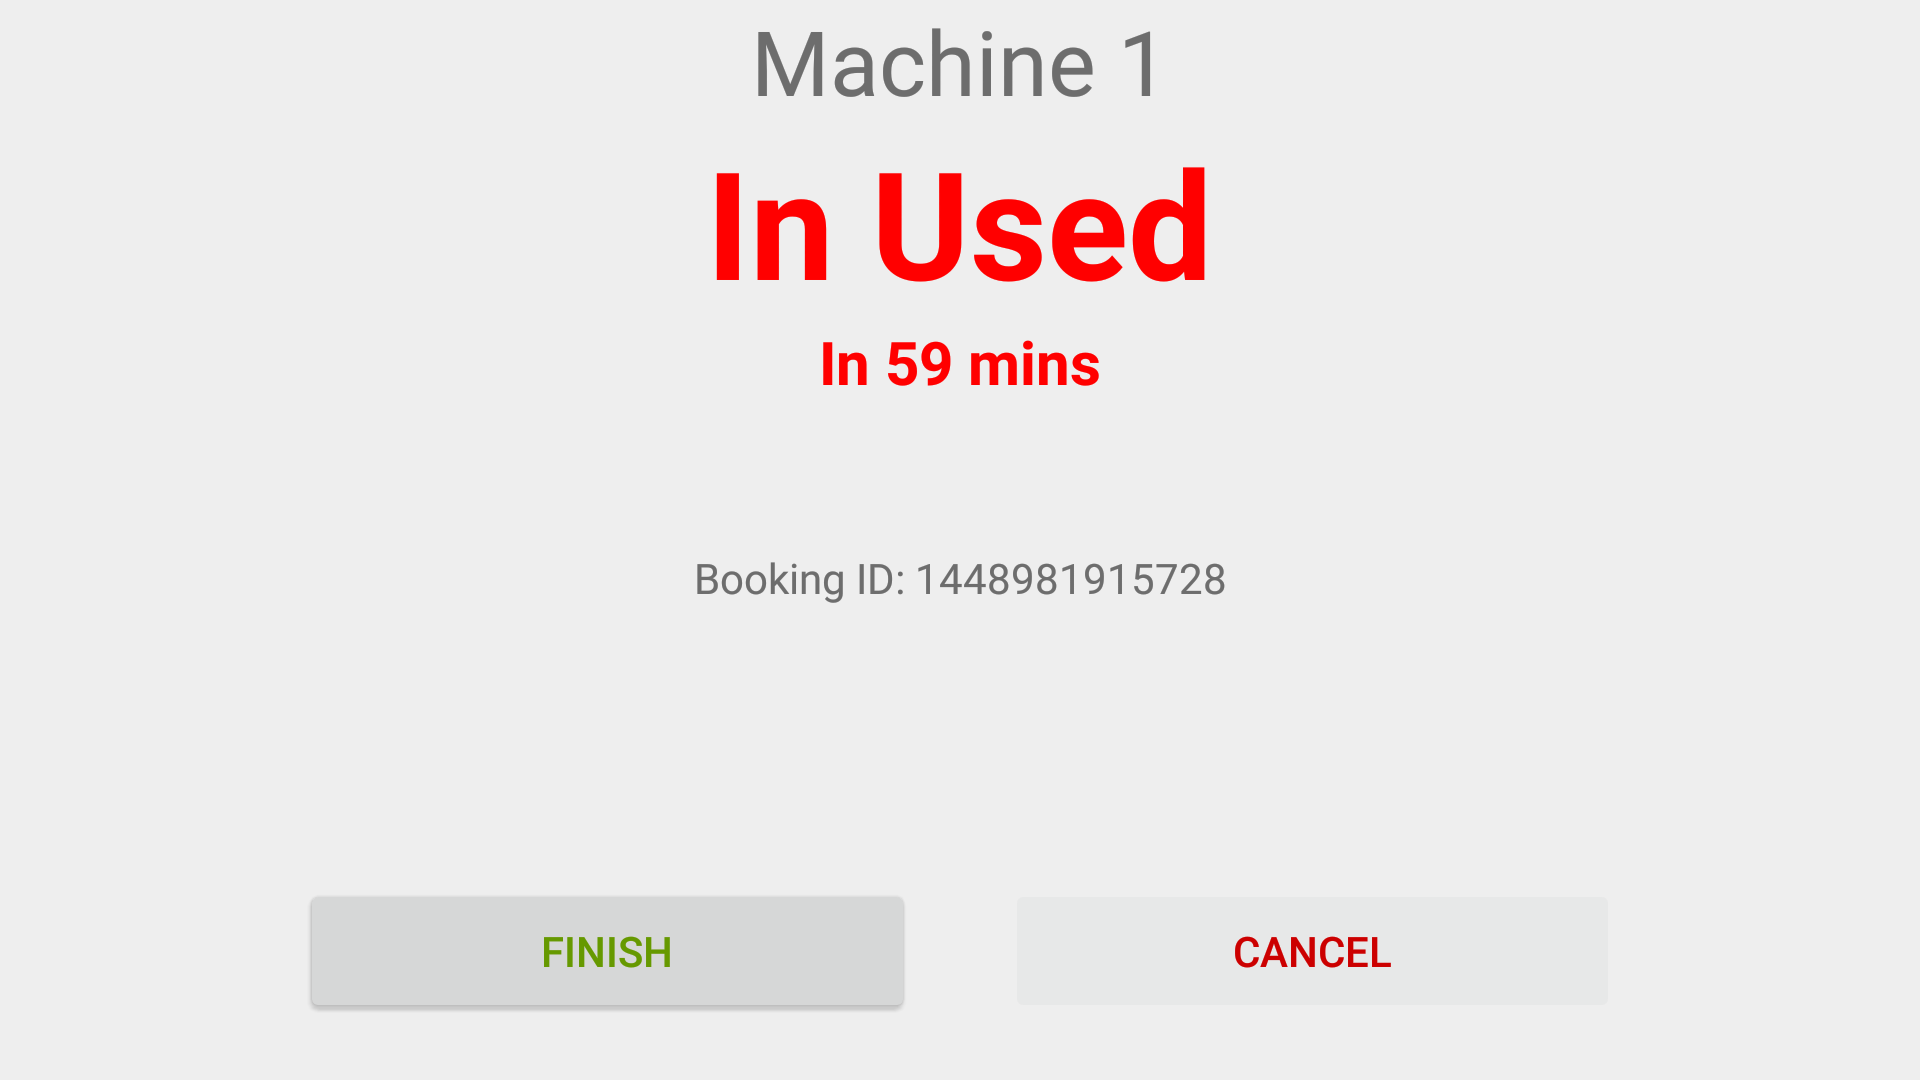
\includegraphics[width=0.8\columnwidth]{figures/inuse}
  \caption{Monitoring display when the machine is running.}~\label{fig:figure3}
\end{figure}
\subsubsection{{\toolname} Application}
{\toolname} is an Android application which allows users to reserve a washing machine, manage booking, observe the current states of the machines, etc. Figure \ref{fig:menu} shows the menu of the application.

The \emph{Booking} tab (see Figure \ref{fig:booking}) allows users to make a reservation for a specific time-slot. There is limitation on the number of time-slots user could book in a week. This number would increase when user get to higher level. Figure \ref{fig:hours} shows the booking interface with time-slots. Users would be awarded points for each time-slot they reserve. The amounts of awards depend on how popular that time-slot is.
\begin{figure*}%
    \centering
    \subfloat[Main menu]{{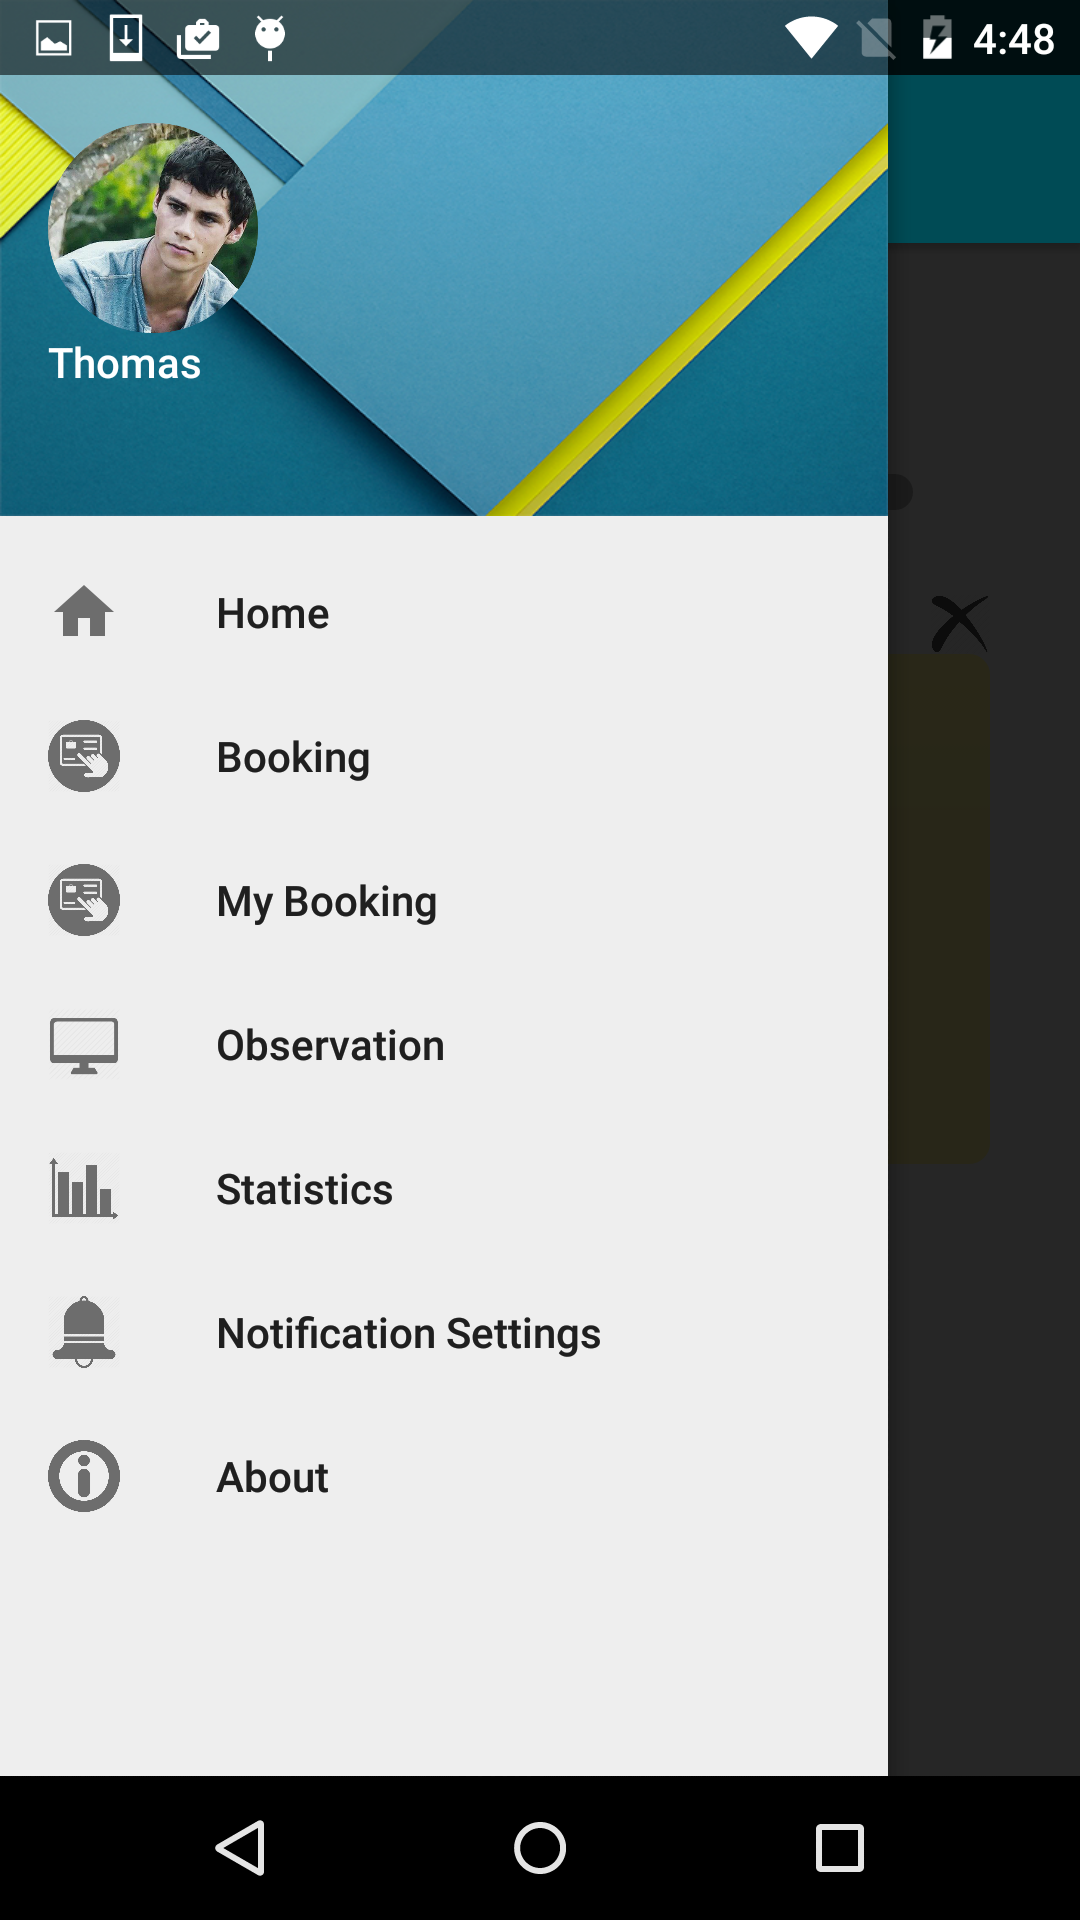
\includegraphics[width=0.4\columnwidth]{figures/menu} \label{fig:menu}}}
    %\qquad
    \subfloat[Home]{{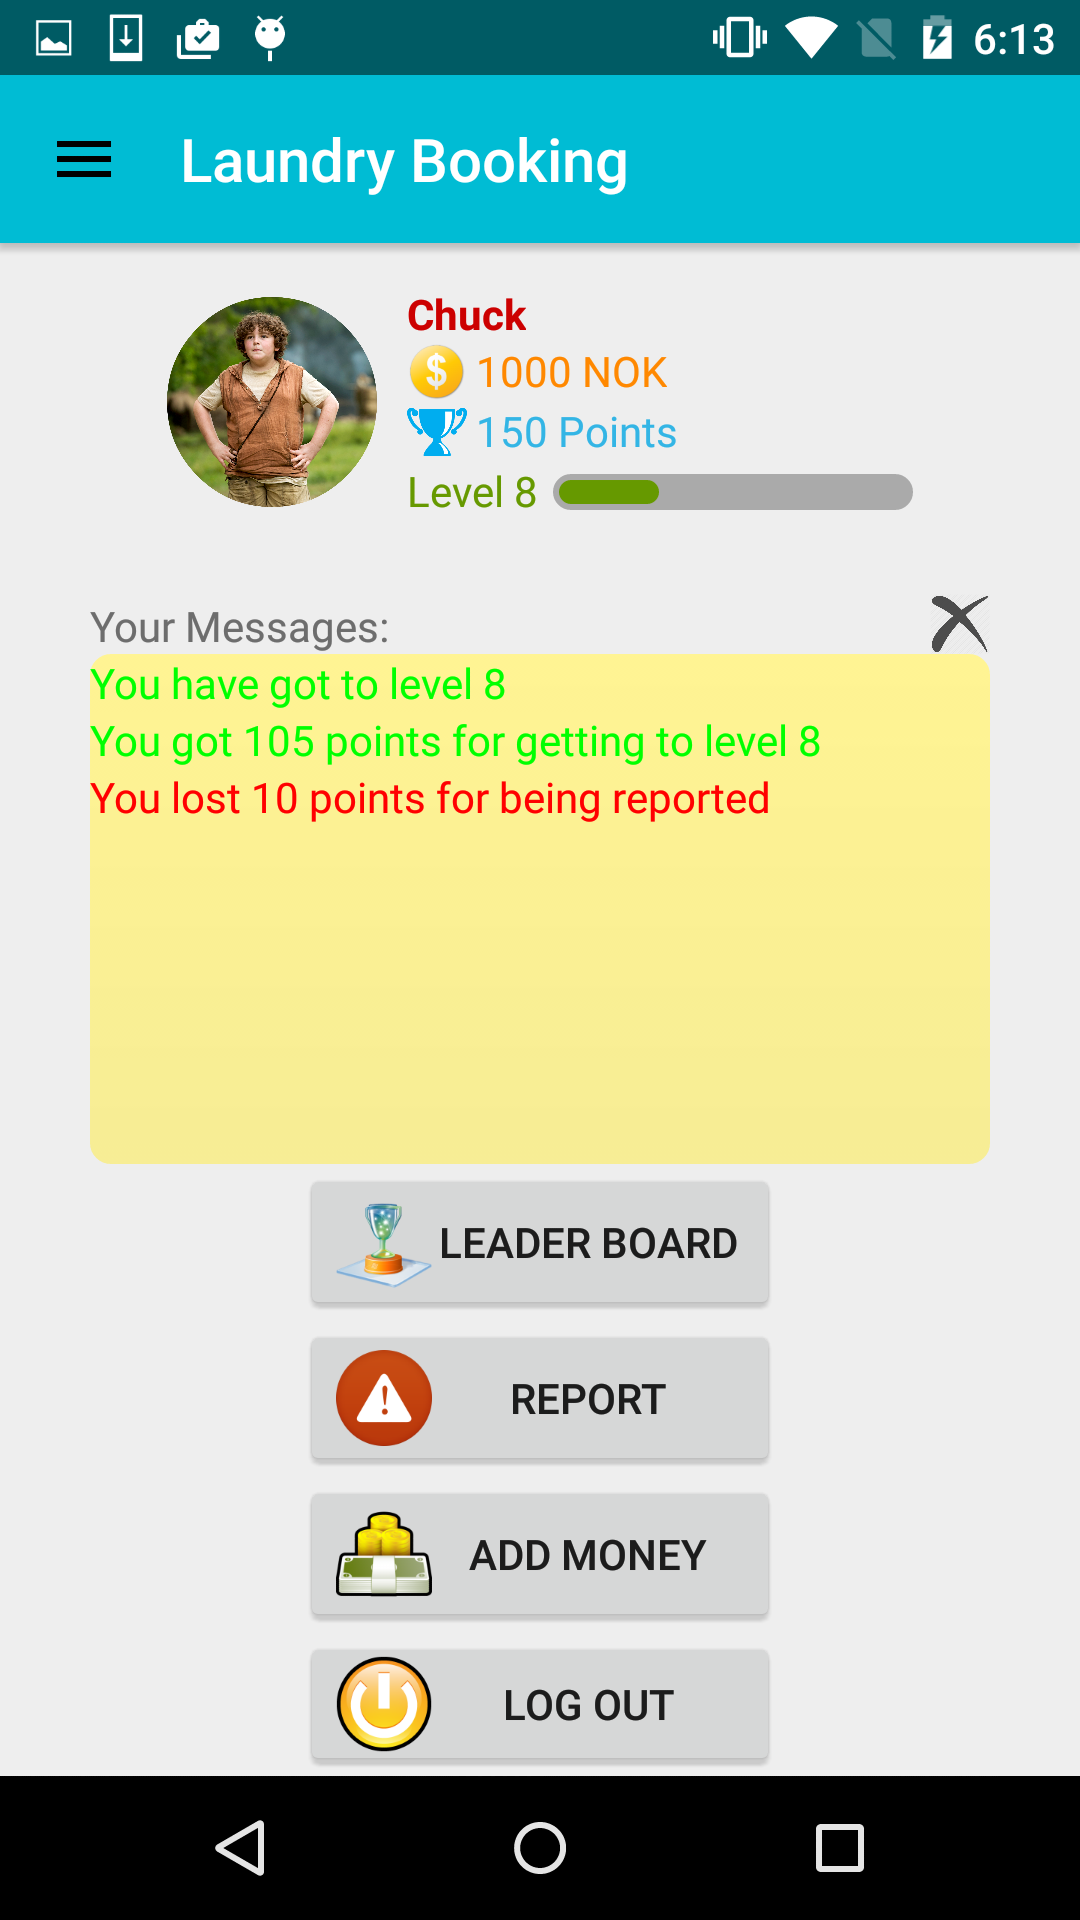
\includegraphics[width=0.4\columnwidth]{figures/home} \label{fig:home} }}
		\subfloat[Booking]{{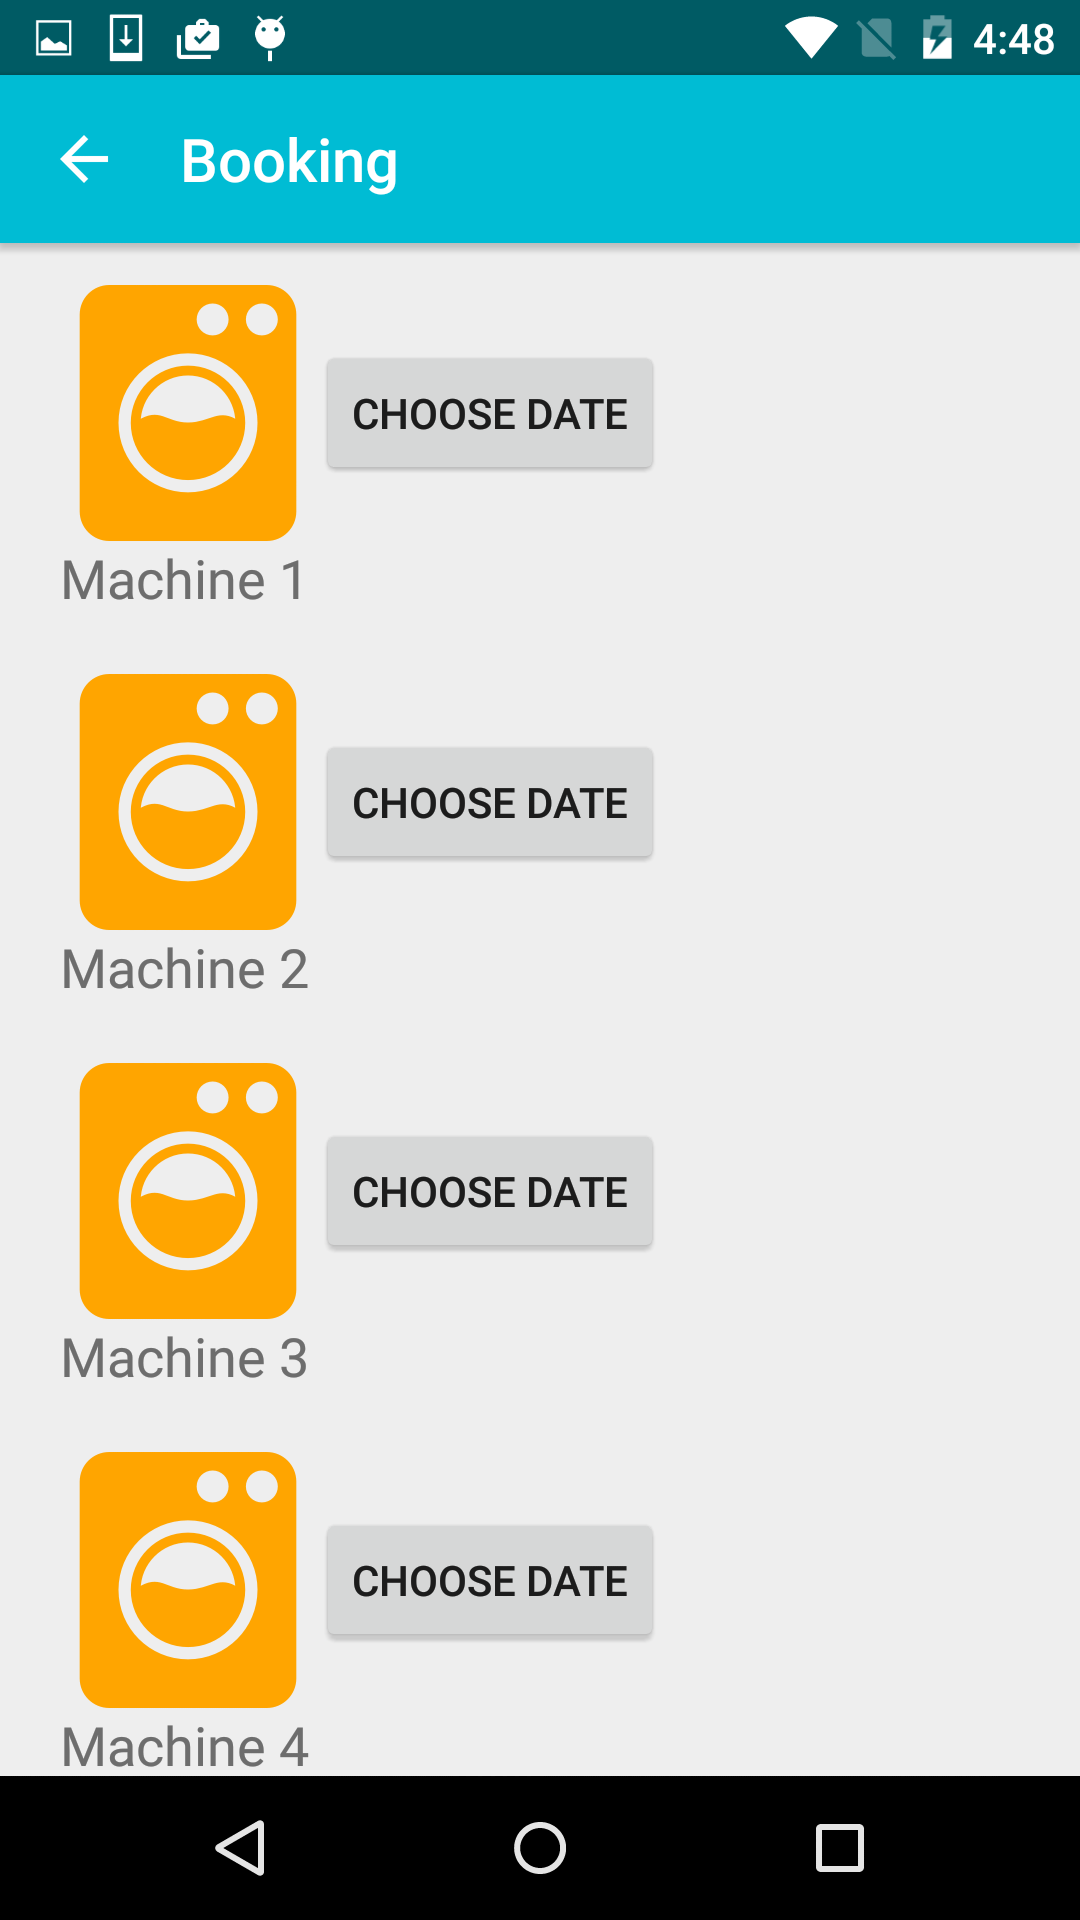
\includegraphics[width=0.4\columnwidth]{figures/booking} \label{fig:booking} }}
		\subfloat[Observation]{{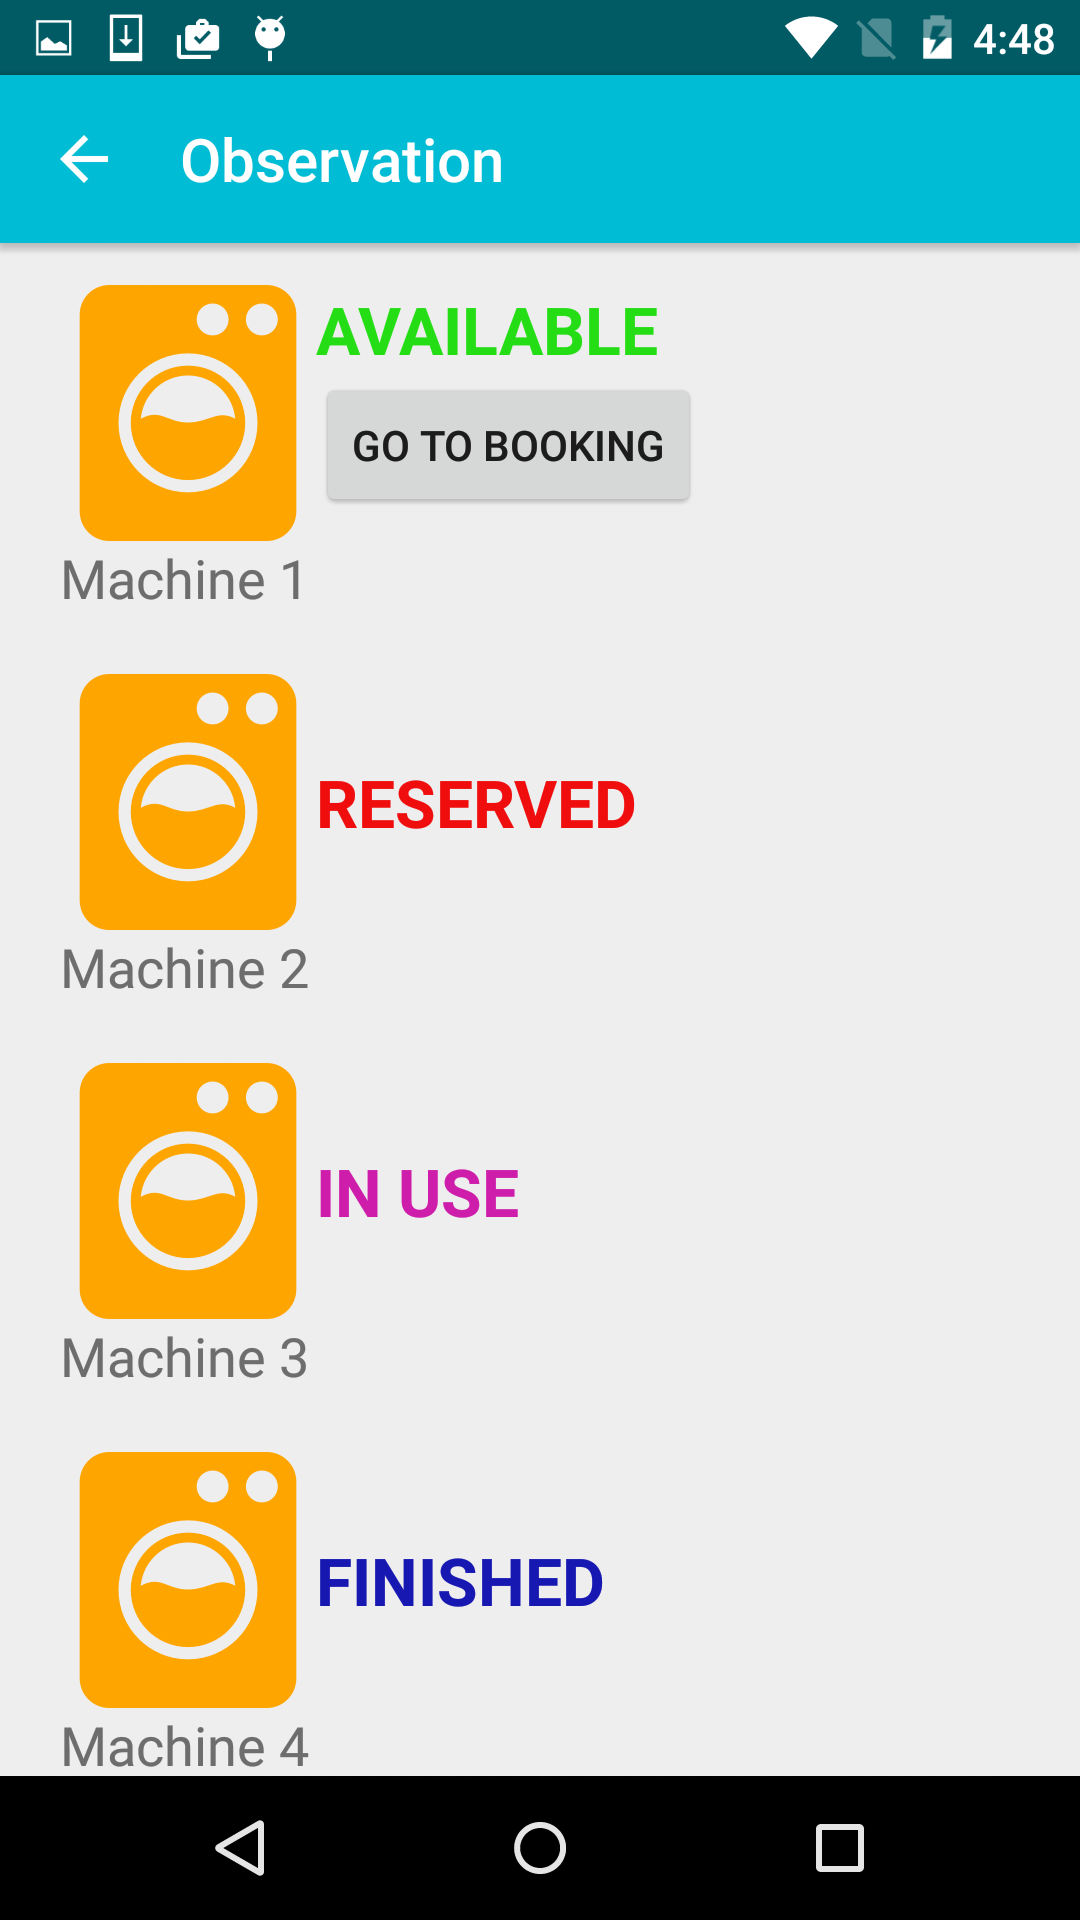
\includegraphics[width=0.4\columnwidth]{figures/observation} \label{fig:observation} }}
		\subfloat[Statistics]{{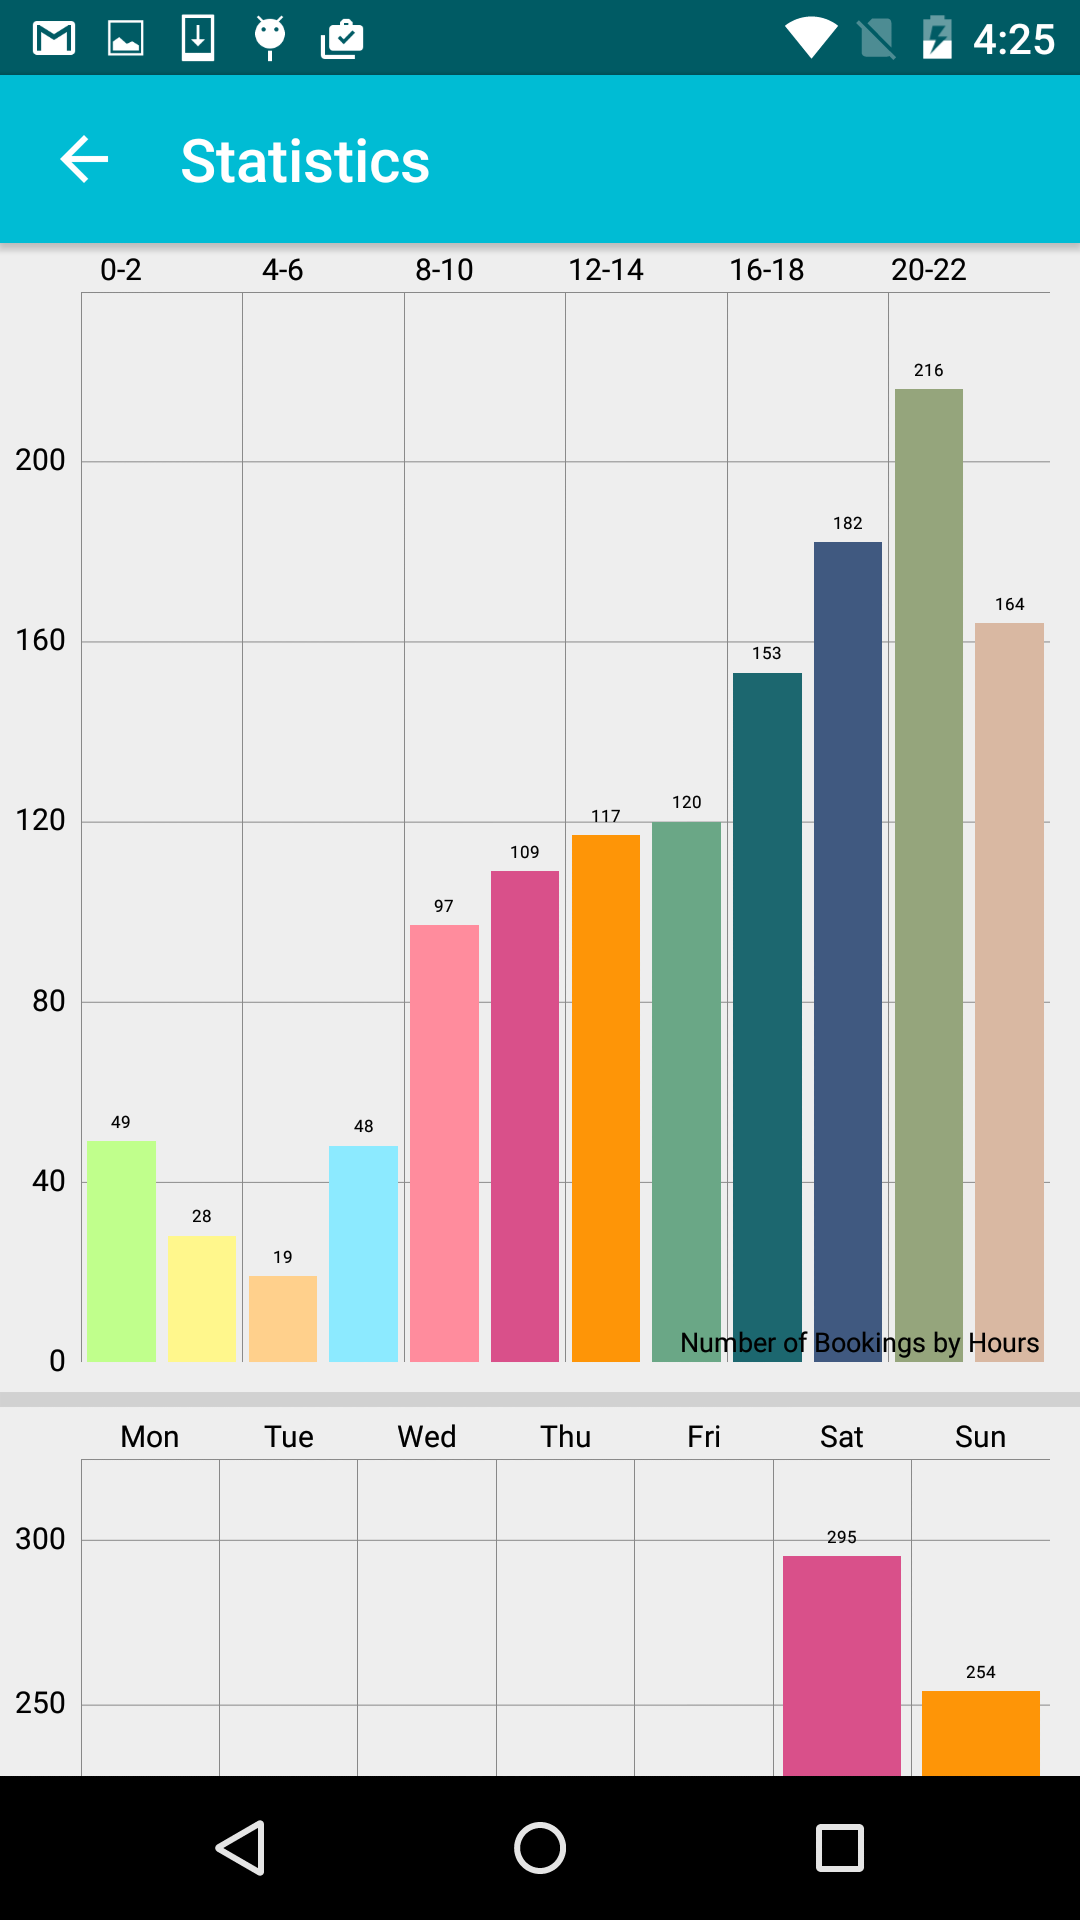
\includegraphics[width=0.4\columnwidth]{figures/stat} \label{fig:stat} }}
    \caption{User interface of \toolname.}%
    \label{fig:figure4}
\end{figure*}

In \emph{My Booking} tab, users could find all their upcoming bookings. They could also cancel a booking in this tab.

 \emph{Observation} (see Figure \ref{fig:observation}) shows the current states of all washing machine. Users could use this function to check for available machines at that moment and use it right away without booking in advance.

There are two bar charts displayed in \emph{Statistics} tab (see Figure \ref{fig:stat}). The first one illustrates numbers of bookings in previous week by hours while the second one represents these numbers by days. Users could use these statistics to plan their ``laundry strategy'' of the week.

\emph{Notification} allows users to set reminders. The application always use in-app notification to remind users for upcoming bookings or finished jobs. In addition, they could choose to set reminder by email or SMS message.
\begin{figure}[h]%
    \centering
    \subfloat[Time-slots and award points]{{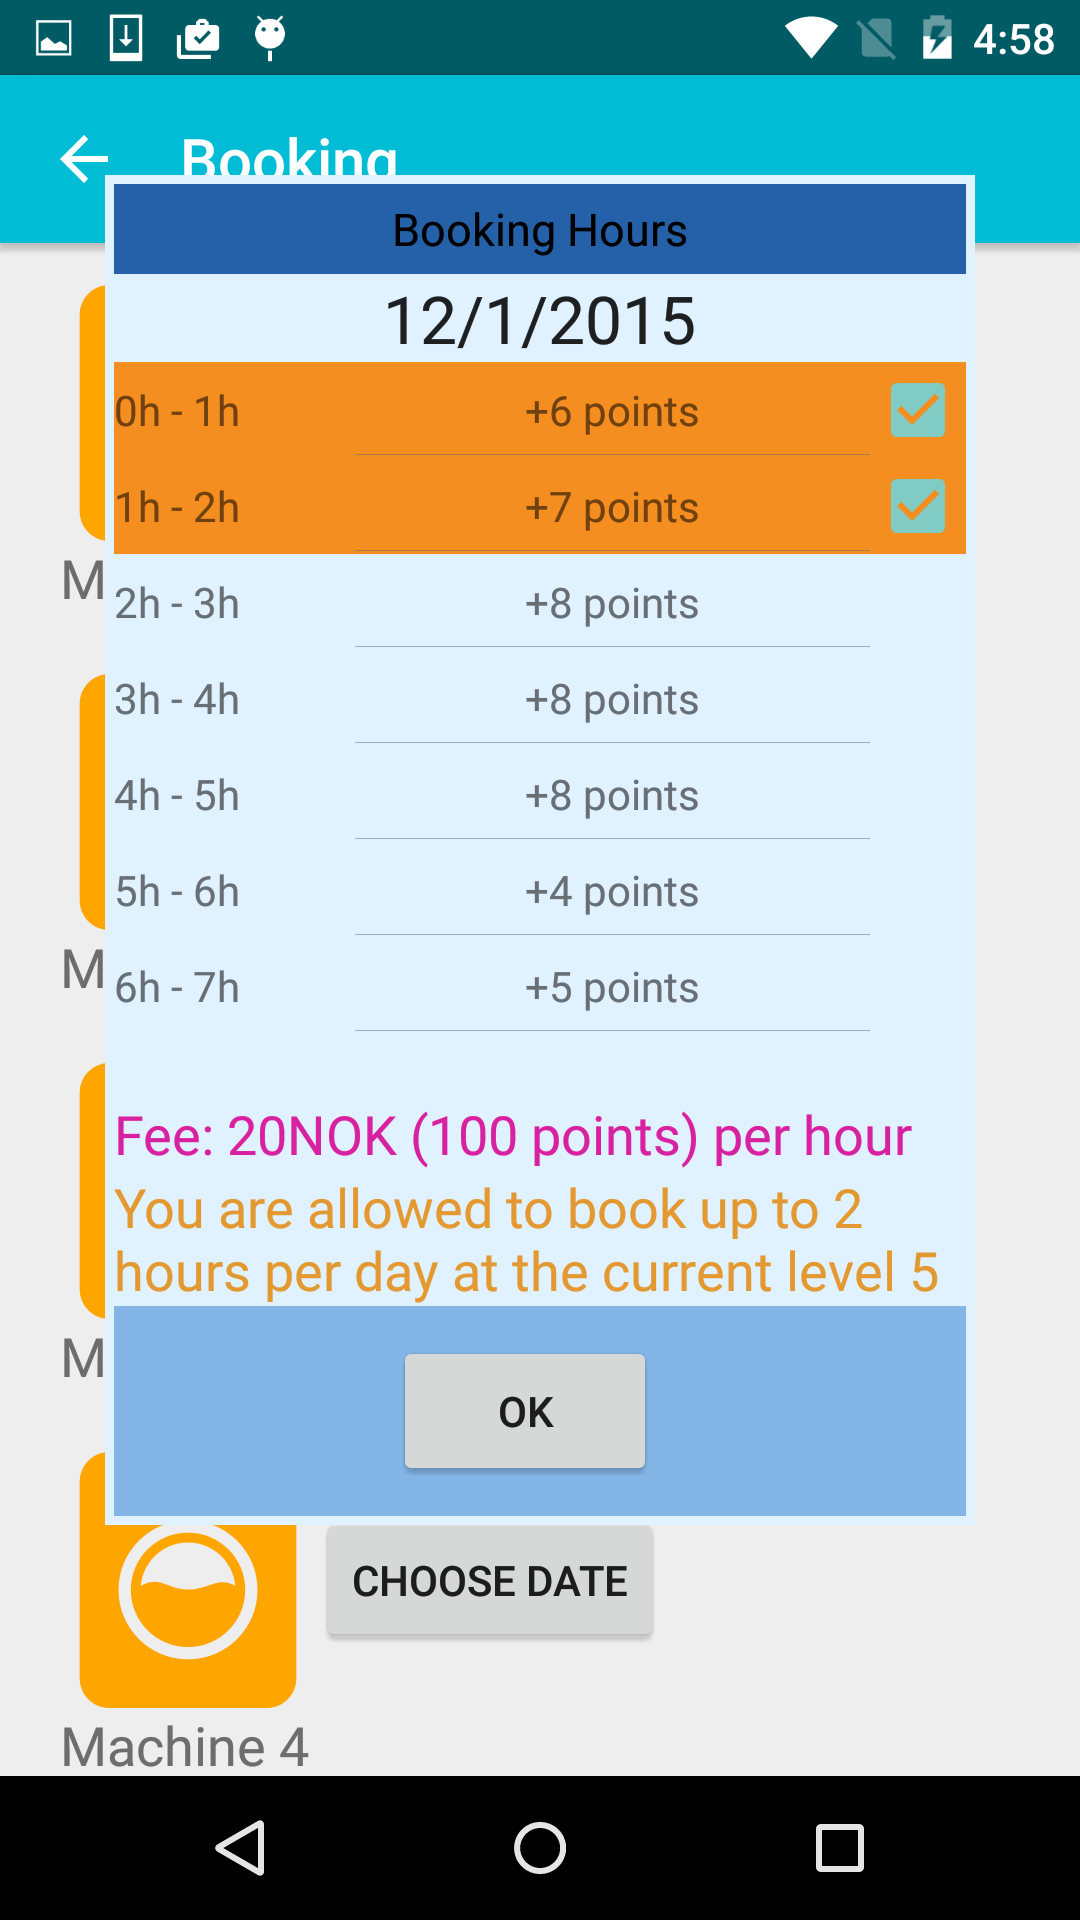
\includegraphics[width=0.4\columnwidth]{figures/hours} \label{fig:hours}}}
    %\qquad
    \subfloat[Leader Board]{{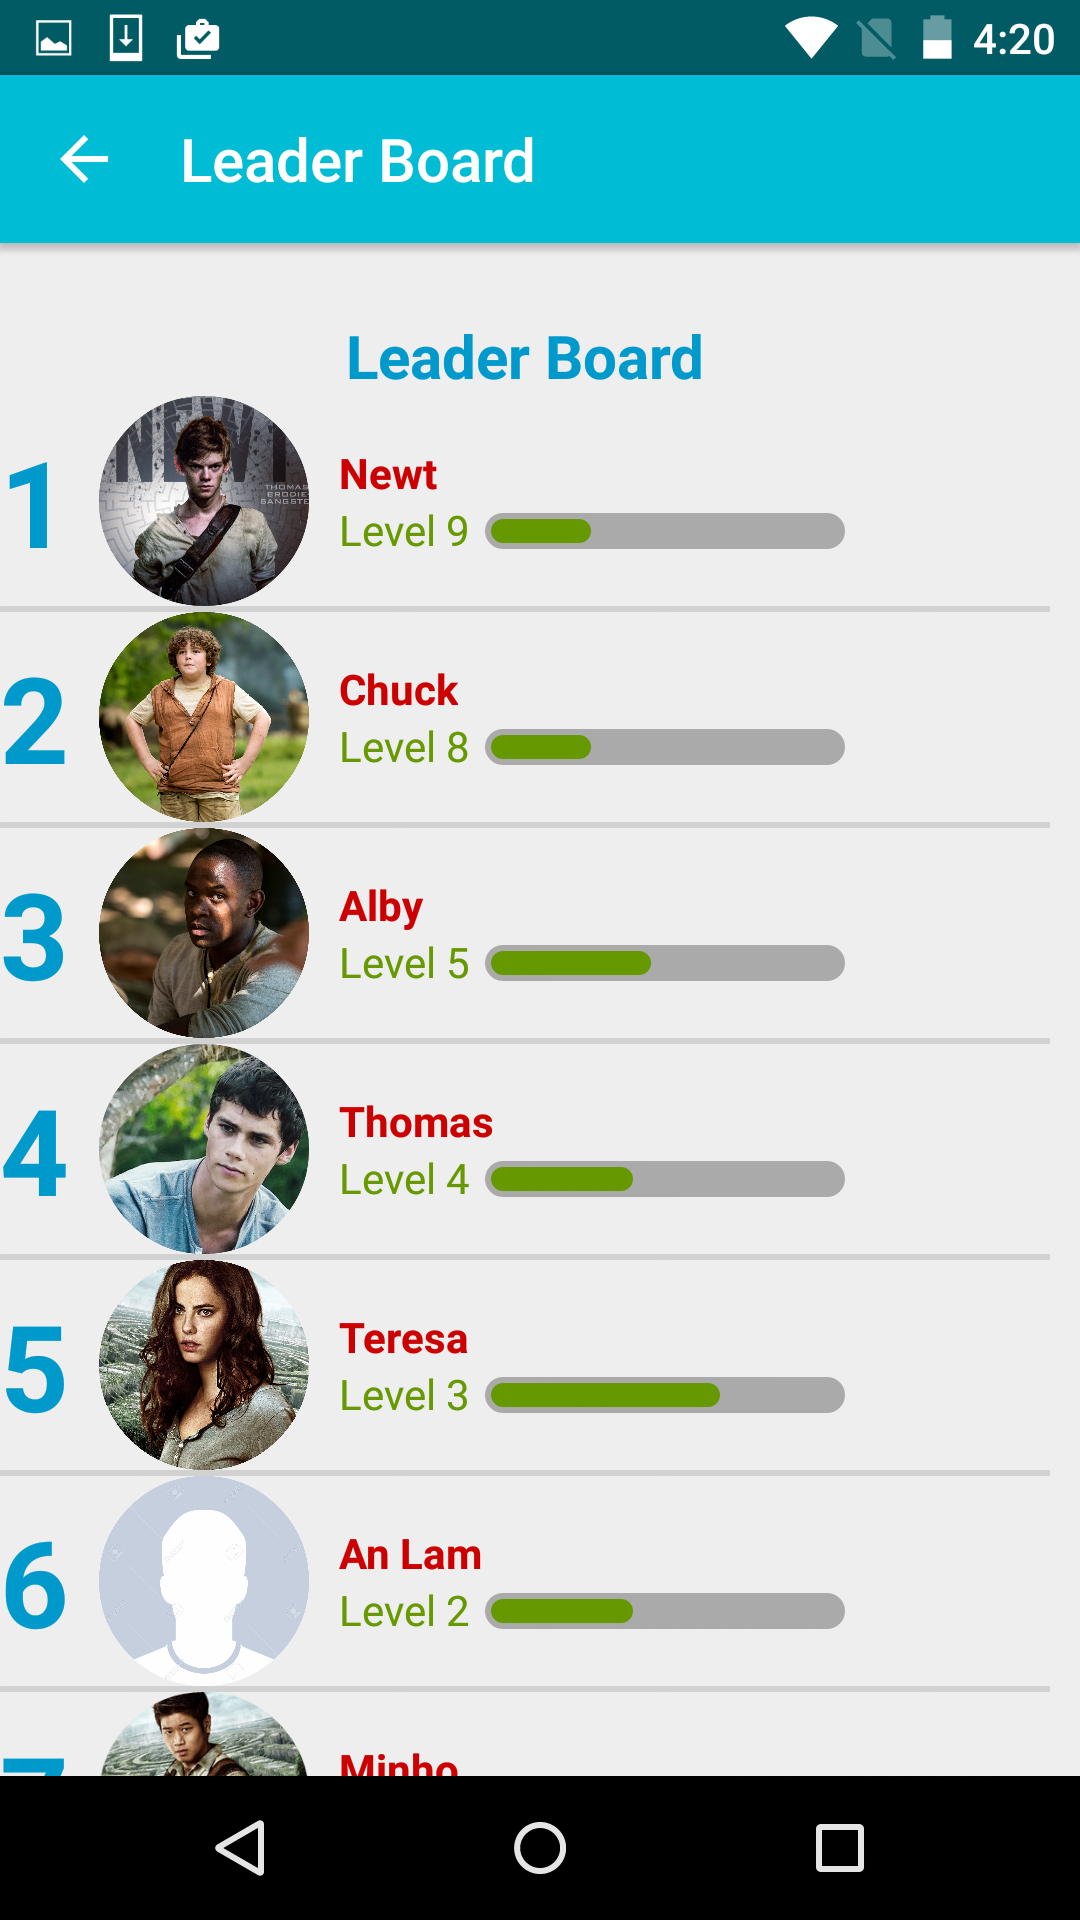
\includegraphics[width=0.4\columnwidth]{figures/leaderboard} \label{fig:leaderboard} }}
		\caption{Time-slots and Leader board.}%
    \label{fig:figure5}
\end{figure}

The \emph{Home} interface (see Figure \ref {fig:home}) displays all information about the user. This is where gamification idea is implemented. In this tab, users could find their avatars, names,  balance and points, levels and progression as well as messages about their activities. There are also buttons allowing them to access leader board (see Figure \ref{fig:leaderboard}), report a person or add money to their accounts. 

\section{Evaluation}

Evaluation

\section{Conclusion}

Conclusion

% Balancing columns in a ref list is a bit of a pain because you
% either use a hack like flushend or balance, or manually insert
% a column break.  http://www.tex.ac.uk/cgi-bin/texfaq2html?label=balance
% multicols doesn't work because we're already in two-column mode,
% and flushend isn't awesome, so I choose balance.  See this
% for more info: http://cs.brown.edu/system/software/latex/doc/balance.pdf
%
% Note that in a perfect world balance wants to be in the first
% column of the last page.
%
% If balance doesn't work for you, you can remove that and
% hard-code a column break into the bbl file right before you
% submit:
%
% http://stackoverflow.com/questions/2149854/how-to-manually-equalize-columns-
% in-an-ieee-paper-if-using-bibtex
%
% Or, just remove \balance and give up on balancing the last page.
%
%\balance{}

% REFERENCES FORMAT
% References must be the same font size as other body text.
\bibliographystyle{SIGCHI-Reference-Format}
\bibliography{ref}

\end{document}

%%% Local Variables:
%%% mode: latex
%%% TeX-master: t
%%% End:
